\chapter{Örnekleme Dağılımları}
\label{ch:sampling-distributions}

\begin{hedefler}
Bu bölümün sonunda:
\begin{itemize}
  \item örnekleme değişkenliği ile yanlılığı ayırabilecek,
  \item ham veri dağılımı ile örnekleme dağılımını karşılaştırabilecek,
  \item örneklem ortalaması ve oranının merkezini ve standart hatasını açıklayabilecek,
  \item bir örnekleme dağılımını tam sayım veya benzetimle oluşturabileceksiniz.
\end{itemize}
\end{hedefler}

\begin{prerequisitebox}
Evren, örneklem, parametre, istatistik, ortalama, oran ve varyans kavramları
hatırlanmalıdır. Basit olasılık ve beklenen değer bilgisi yararlıdır.
\end{prerequisitebox}

\begin{hazirlik}
Aynı evrenden aynı yöntemle seçilen iki örneklemin ortalamaları farklıysa bu
durum mutlaka veri hatası veya yanlılık mıdır? Rastgele değişkenlikle ayırın.
\end{hazirlik}

Evren, örneklem, parametre ve istatistik ayrımı için
Bölüm~\ref{sec:population-parameter}; merkez ve varyans özetleri için
Bölüm~\ref{ch:descriptive} kullanılabilir.

\section{Örnekleme değişkenliği}

Aynı evrenden aynı yöntemle seçilen iki örneklem genellikle aynı birimleri
içermez. Bu nedenle örneklem ortalaması, oranı veya korelasyonu örneklemden
örnekleme değişir. Bu doğal değişime \emph{örnekleme değişkenliği} denir.
Örnekleme değişkenliği hata yapılmış olması anlamına gelmez; olasılıklı
örneklemenin beklenen bir sonucudur.

\section{İstatistik ve örnekleme dağılımı}
\label{sec:sampling-distribution}

\begin{definitionbox}
Bir örneklem istatistiğinin, aynı örnekleme süreci çok kez tekrarlandığında
alabileceği değerlerin olasılık dağılımına \emph{örnekleme dağılımı} denir.
Örneğin her tekrarda $n$ gözlem seçilip $\bar X$ hesaplanırsa elde edilen
ortalamaların dağılımı $\bar X$'ın örnekleme dağılımıdır.
\end{definitionbox}
Örnekleme
dağılımları ve beklenen değer sonuçlarının ayrıntılı kuramsal sunumu için
\citet{hogg2015} incelenebilir.

Bağımsız ve aynı dağılımlı gözlemler için
\[
\E[\bar X]=\mu,
\qquad
\Var(\bar X)=\frac{\sigma^2}{n}.
\]
Bu sonuç, örneklem ortalamasının merkezinin evren ortalaması olduğunu ve
örneklem hacmi arttıkça dağılımının daraldığını gösterir.

Örneklem oranı için de benzer bir yapı vardır. Başarı olasılığı $p$ olan
bağımsız Bernoulli gözlemlerinde
\[
\E[\hat p]=p,
\qquad
\Var(\hat p)=\frac{p(1-p)}{n},
\qquad
\SE(\hat p)=\sqrt{\frac{p(1-p)}{n}}.
\]
Bu eşitlikler, ortalama ve oran gibi farklı istatistiklerin aynı temel
çıkarım mantığıyla incelenebildiğini gösterir.

\section{Tam sayımlı çözümlü örnek}

Değerleri $2,4,6,8$ olan dört elemanlı bir evrenden, yerine koyarak ve sıralı
biçimde iki gözlem seçilsin. Evren ortalaması $\mu=5$, evren varyansı
$\sigma^2=5$'tir. Olası $4^2=16$ örneklemin ortalamaları aşağıdaki dağılımı
oluşturur.

\begin{table}[H]
\centering
\caption{$n=2$ için örneklem ortalamasının tam örnekleme dağılımı.}
\label{tab:exact-sampling-distribution}
\begin{tabular}{lrrrrrrr}
\toprule
$\bar x$ & 2 & 3 & 4 & 5 & 6 & 7 & 8 \\
\midrule
Frekans & 1 & 2 & 3 & 4 & 3 & 2 & 1 \\
Olasılık & $1/16$ & $2/16$ & $3/16$ & $4/16$ & $3/16$ & $2/16$ & $1/16$ \\
\bottomrule
\end{tabular}
\end{table}

Tablo~\ref{tab:exact-sampling-distribution}'deki dağılımın beklenen değeri 5,
varyansı ise $5/2=2{,}5$'tir. Tek tek evren
değerleri eşit sıklıkta görünmesine rağmen örneklem ortalamaları merkezde daha
çok toplanmıştır.

\begin{figure}[H]
\centering
\begin{tikzpicture}[x=0.85cm,y=0.46cm]
  \draw[->,PrismGray] (1.4,0) -- (8.7,0);
  \draw[->,PrismGray] (1.4,0) -- (1.4,5.5);
  \foreach \x in {2,...,8} \node[below,font=\scriptsize] at (\x,0) {\x};
  \foreach \x in {2,4,6,8}
    \fill[PrismWarnOrange!85!black] (\x-0.22,0) rectangle (\x+0.22,1);
  \node[anchor=west,font=\scriptsize] at (8.8,1.0) {evren değerleri};

  \begin{scope}[yshift=-4.3cm]
    \draw[->,PrismGray] (1.4,0) -- (8.7,0);
    \draw[->,PrismGray] (1.4,0) -- (1.4,5.5);
    \foreach \x in {2,...,8} \node[below,font=\scriptsize] at (\x,0) {\x};
    \foreach \x/\h in {2/1,3/2,4/3,5/4,6/3,7/2,8/1}
      \fill[PrismBlue!78] (\x-0.22,0) rectangle (\x+0.22,\h);
    \node[anchor=west,font=\scriptsize] at (8.8,2.0) {$\bar X$ dağılımı};
  \end{scope}
\end{tikzpicture}
\caption{Ham evren değerleri ile örneklem ortalamasının dağılımı.}
\label{fig:raw-vs-sampling}
\end{figure}

\section{Ham veri dağılımı ile örnekleme dağılımı}

Şekil~\ref{fig:raw-vs-sampling}'de üst ve alt panellerin ayrılması bu iki
dağılımın farklı analiz birimlerine dayandığını vurgular. Ham veri dağılımı
bireyler arasındaki farklılığı gösterir. Örnekleme dağılımı
ise bir istatistiğin farklı örneklemlerdeki değişkenliğini gösterir. Tek bir
örneklemdeki puan histogramı, ortalamanın örnekleme dağılımı değildir.

\begin{mistakebox}
Örneklem hacmi arttığında bireysel puanların değişkenliği zorunlu olarak
azalmaz. Azalan nicelik, örneklem ortalaması gibi tahminlerin örneklemden
örnekleme değişkenliğidir.
\end{mistakebox}

\section{Benzetimle örnekleme dağılımı}
\label{sec:sampling-simulation}

Bir evrenden tekrar tekrar örnek seçmek, her örneklemde aynı istatistiği
hesaplamak ve sonuçların histogramını çizmek örnekleme dağılımını görünür
kılar. Benzetim, tahminlerin tek bir veri setine özgü olmadığını ve çıkarımın
tekrarlı örnekleme mantığına dayandığını gösterir.

Benzetim sonuçları üç soruyla değerlendirilmelidir: Dağılımın merkezi hedef
parametreye yakın mı? Dağılımın genişliği kuramsal standart hataya yakın mı?
Örneklem hacmi arttığında biçim ve genişlik nasıl değişiyor? Tek bir benzetim
sonucu kanıt değildir; tekrar sayısı artırıldığında Monte Carlo dalgalanması
azalmalıdır. Şekil~\ref{fig:sampling-size-narrowing}, son sorunun görsel
karşılığını verir.

\begin{figure}[H]
\centering
\begin{tikzpicture}[x=0.34cm,y=0.38cm]
  \foreach \shift/\label in {0/{$n=5$},3.9/{$n=25$},7.8/{$n=100$}} {
    \begin{scope}[xshift=\shift cm]
      \draw[->,PrismGray] (-0.4,0)--(8.7,0);
      \node[below,font=\scriptsize] at (4.1,-0.2) {\label};
      \node[below,font=\tiny] at (0,0) {30};
      \node[below,font=\tiny] at (4,0) {50};
      \node[below,font=\tiny] at (8,0) {70};
    \end{scope}
  }
  \foreach \x/\h in {0/0.6,1/1.2,2/2.1,3/3.0,4/3.4,5/3.0,6/2.1,7/1.2,8/0.6}
    \fill[PrismSubheadingBlue!58] (\x-0.38,0) rectangle (\x+0.38,\h);
  \begin{scope}[xshift=3.9cm]
    \foreach \x/\h in {1/0.1,2/0.5,3/2.2,4/4.6,5/2.2,6/0.5,7/0.1}
      \fill[PrismSubheadingBlue!72] (\x-0.38,0) rectangle (\x+0.38,\h);
  \end{scope}
  \begin{scope}[xshift=7.8cm]
    \foreach \x/\h in {2/0.1,3/1.0,4/5.3,5/1.0,6/0.1}
      \fill[PrismBlue!82] (\x-0.38,0) rectangle (\x+0.38,\h);
  \end{scope}
  \draw[PrismWarnOrange!85!black,dashed] (4,-0.1)--(4,5.7);
  \draw[PrismWarnOrange!85!black,dashed] ([xshift=3.9cm]4,-0.1)--([xshift=3.9cm]4,5.7);
  \draw[PrismWarnOrange!85!black,dashed] ([xshift=7.8cm]4,-0.1)--([xshift=7.8cm]4,5.7);
\end{tikzpicture}
\caption{Aynı evrenden benzetilen örneklem ortalamalarının $n$ arttıkça daralması.}
\label{fig:sampling-size-narrowing}
\end{figure}

\section{Sayısal bir karşılaştırma}

Ortalaması $\mu=50$, standart sapması $\sigma=10$ olan bir evrenden
$n=25$ birimlik örneklemler seçilsin. Tek tek gözlemlerin standart sapması
10 iken örneklem ortalamalarının standart sapması
\[
\SE(\bar X)=\frac{10}{\sqrt{25}}=2
\]
olur. Dolayısıyla örneklem ortalamalarının çoğu 50 çevresinde, bireysel
puanlardan çok daha dar bir bölgede toplanır. Örneklem hacmi $n=100$ olursa
bu değer 1'e düşer. Merkez değişmemiş, yalnız tahminin örneklemeden gelen
belirsizliği azalmıştır.

\Needspace{20\baselineskip}
\begin{softwarebox}
Aşağıdaki benzetim, normal bir evrenden 5000 kez örnek seçerek her örneklemin
ortalamasını saklar. Son satırdaki standart sapma kuramsal değer olan 2'ye
yaklaşmalıdır.
\begin{lstlisting}
import numpy as np
import matplotlib.pyplot as plt

rng = np.random.default_rng(2026)
means = rng.normal(50, 10, size=(5000, 25)).mean(axis=1)
print(means.mean(), means.std(ddof=1))
plt.hist(means, bins=30, density=True,
         color="#8FB8D8", edgecolor="white")
plt.axvline(50, color="#1F4E79", linewidth=2)
plt.xlabel("Orneklem ortalamasi")
plt.ylabel("Yogunluk")
plt.show()
\end{lstlisting}
Tohum değerinin yazılması analizin yeniden üretilebilmesini sağlar; kullanılan
rassal sayı altyapısı NumPy içinde belgelenmiştir \citep{harris2020}.
\end{softwarebox}

\section{Yanlılık ile değişkenliği ayırmak}
\label{sec:sampling-bias-variance}

Örnekleme dağılımının merkezi hedef parametreden sistematik olarak uzaksa
yanlılık, dağılım genişse yüksek örnekleme değişkenliği söz konusudur. Büyük
örneklem değişkenliği azaltabilir; fakat kapsam hatası veya yanıtlamama gibi
sistematik yanlılıkları kendiliğinden gidermez.

\begin{assumptionbox}
Standart hata formülü gözlemlerin bağımsız ve aynı dağılımdan geldiği basit
modeli temel alır. Küme örneklemesi, zaman içinde tekrarlı ölçümler veya aynı
sınıftaki öğrencilerin birbirine benzemesi bağımsızlığı zayıflatabilir. Böyle
durumlarda tasarıma uygun standart hata yöntemleri gerekir.
\end{assumptionbox}

\section{Çözümlü problemler}

\subsection*{Problem 1: Örneklem hacmi ve ortalamanın standart hatası}

Ortalaması 70, standart sapması 12 olan bir puan evreninden önce $n=36$,
sonra $n=144$ büyüklüğünde bağımsız örneklemler seçilecektir. İki durumda
örneklem ortalamasının beklenen değerini, varyansını ve standart hatasını
bulun.

\textbf{Çözüm.} Örneklem ortalamasının merkezi örneklem hacminden bağımsız
olarak evren ortalamasıdır:
\[
\E[\bar X]=\mu=70.
\]
$n=36$ için
\[
\Var(\bar X)=\frac{12^2}{36}=4,
\qquad \SE(\bar X)=\frac{12}{\sqrt{36}}=2.
\]
$n=144$ için ise
\[
\Var(\bar X)=\frac{12^2}{144}=1,
\qquad \SE(\bar X)=\frac{12}{\sqrt{144}}=1.
\]
Örneklem hacmi dört katına çıktığında standart hata yarıya, varyans dörtte
bire düşmüştür. Dağılımın merkezi değişmemiş; örneklem ortalamasının olası
değerleri 70 çevresinde daha sıkı toplanmıştır.

\textbf{Sık hata.} $n$ dört katına çıktığında standart hata dörtte bire
düşmez. Standart hata $1/\sqrt n$, varyans ise $1/n$ oranında değişir.

\subsection*{Problem 2: Küçük bir evrende tam örnekleme dağılımı}

Değerleri $1,3,5$ olan bir evrenden yerine koyarak ve sıralı biçimde iki
gözlem seçilsin. Örneklem ortalamasının alabileceği değerleri ve olasılıklarını
bulun; dağılımın beklenen değerini ve varyansını doğrulayın.

\textbf{Çözüm.} Olası $3^2=9$ sıralı örneklem vardır. Ortalamaların dağılımı
şöyledir:

\begin{center}
\begin{tabular}{lrrrrr}
\toprule
$\bar x$ & 1 & 2 & 3 & 4 & 5 \\
\midrule
Frekans & 1 & 2 & 3 & 2 & 1 \\
Olasılık & $1/9$ & $2/9$ & $3/9$ & $2/9$ & $1/9$ \\
\bottomrule
\end{tabular}
\end{center}

Evren ortalaması $\mu=(1+3+5)/3=3$ ve evren varyansı
\[
\sigma^2=\frac{(1-3)^2+(3-3)^2+(5-3)^2}{3}=\frac{8}{3}
\]
olur. Örnekleme dağılımından doğrudan hesaplandığında
\[
\E[\bar X]=3,
\qquad \Var(\bar X)=\frac{4}{3}
\]
elde edilir. Kuramsal formül de aynı sonucu verir:
\[
\Var(\bar X)=\frac{\sigma^2}{n}
=\frac{8/3}{2}=\frac{4}{3}.
\]
Örneklem ortalamaları evren ortalamasında merkezlenmiş ve uç değerlere göre
merkezde daha yoğun toplanmıştır.

\subsection*{Problem 3: Örneklem oranının değişkenliği}

Bir eğitim platformundaki öğrencilerin yüzde 30'unun bir modülü tamamladığı
varsayılsın. $n=400$ büyüklüğündeki rastgele örneklemlerde tamamlayanların
oranının standart hatasını bulun. Örneklem hacmi 1.600'e çıkarılırsa sonuç
nasıl değişir?

\textbf{Çözüm.} $p=0{,}30$ ve $1-p=0{,}70$ için
\[
\SE(\hat p)=\sqrt{\frac{0{,}30(0{,}70)}{400}}
=\sqrt{0{,}000525}\approx0{,}0229.
\]
Bu değer yaklaşık 2,29 yüzde puandır. $n=1600$ olduğunda
\[
\SE(\hat p)=\sqrt{\frac{0{,}21}{1600}}
\approx0{,}0115
\]
olur. Örneklem hacmi dört katına çıktığı için standart hata yaklaşık yarıya
inmiştir. İlk tasarımda örneklem oranlarının önemli bir bölümü $0{,}30$
çevresinde yaklaşık $\pm2(0{,}0229)$ aralığında dalgalanırken ikinci tasarımda
bu tipik dalgalanma daha dardır.

\textbf{Yorum.} Standart hata tek tek öğrencilerin tamamlayıp tamamlamamasını
değil, farklı örneklemlerde hesaplanan tamamlanma oranlarının değişkenliğini
ölçer.

\subsection*{Problem 4: Yanlılık ve değişkenliği ayırma}

Gerçek evren ortalaması 50 olsun. Aynı parametreyi tahmin eden A yönteminin
örnekleme dağılımı 50 merkezli ve standart hatası 4; B yönteminin örnekleme
dağılımı 54 merkezli ve standart hatası 1 olsun. Yöntemleri yanlılık ve
değişkenlik bakımından karşılaştırın.

\textbf{Çözüm.} A yönteminin örnekleme dağılımı gerçek parametre olan 50'de
merkezlendiği için yöntem yansızdır. Ancak standart hatasının 4 olması,
örneklemden örnekleme belirgin değişkenlik gösterdiğini belirtir. B yönteminin
standart hatası yalnız 1 olduğundan tahminleri birbirine yakındır; buna karşın
dağılım 54'te merkezlendiği için yanlılığı
\[
\text{Yanlılık}(B)=54-50=4
\]
birimdir.

B yöntemi tutarlı biçimde yanlış hedefe yakın sonuç üretmektedir. Örneklem
hacmini artırmak B'nin değişkenliğini daha da azaltabilir; fakat seçim veya
ölçüm mekanizmasından gelen dört birimlik sistematik sapmayı zorunlu olarak
gidermez. İyi bir tahmin yöntemi hem küçük yanlılık hem düşük değişkenlik
hedefler.

\subsection*{Problem 5: Benzetim çıktısını değerlendirme}

Ortalaması 70 ve standart sapması 12 olan bir evrenden $n=64$ büyüklüğünde
10.000 örneklem seçilerek ortalamalar kaydedilmiştir. Benzetim ortalamalarının
ortalaması 69,96, standart sapması 1,52 bulunmuştur. Sonuçları kuramsal
değerlerle karşılaştırın.

\textbf{Çözüm.} Kuramsal olarak
\[
\E[\bar X]=70,
\qquad \SE(\bar X)=\frac{12}{\sqrt{64}}=1{,}50
\]
olmalıdır. Benzetim merkezi 69,96 ile 70'e, benzetim standart sapması 1,52
ile 1,50'ye oldukça yakındır. Küçük farklar sınırlı sayıda benzetim tekrarının
oluşturduğu Monte Carlo değişkenliğinden kaynaklanabilir.

Benzetim tekrarını 10.000'den 100.000'e çıkarmak, kuramsal standart hatayı
değiştirmez; yalnız benzetimle hesaplanan özetlerin kuramsal değerlere daha
kararlı biçimde yaklaşmasını sağlar. Buna karşılık her örneklemdeki öğrenci
sayısını artırmak gerçekten $\SE(\bar X)$ değerini azaltır.

\begin{outputguidebox}
Bir benzetim çıktısında tekrar sayısı ile her örneklemin hacmini birbirinden
ayırın. Örneklem hacmi tahminin standart hatasını, tekrar sayısı ise benzetim
sonucundaki Monte Carlo dalgalanmasını etkiler. Dağılımın merkezi, genişliği
ve biçimi kuramsal beklentiyle ayrı ayrı karşılaştırılmalıdır.
\end{outputguidebox}

\section{Literatür verisiyle yazılım uygulamaları}
\label{sec:spss-b04}

\textbf{Amaç ve veri.} \texttt{b04.csv}, \citet{cortez2008data} matematik
notlarının ampirik dağılımından geri koyarak üretilen 2.000 tekrar içerir.
Her tekrarda ilk 5 ve ilk 30 çekimin ortalaması kaydedilmiştir. Bunlar yeni
öğrenci gözlemleri değildir. Sabit tohum 2026'dır; üretim algoritması
\texttt{build\_package.py} içindedir. SPSS, hazır tekrarların dağılımını özetler.


\textbf{Ortak veri.} Doğrulanan B04 uygulamasında üç yazılım da
\nolinkurl{companion/spss/csv/b04.csv} dosyasındaki hazır tekrarları
kullanmıştır. Dosya 2.000 satır ve üç sütun içerir: \texttt{rep},
\texttt{ort5}, \texttt{ort30}. B01'in öğrenci dosyası bu uygulamada
kullanılmaz. Bu karşılaştırma Excel içe aktarmanın doğrulandığı anlamına
gelmez. Kodları \texttt{companion} klasörünü içeren paket kökünden
çalıştırın; veri sözlüğü ve hazırlık için bkz. sayfa~\pageref{sec:spss-guide}.

\subsection{IBM SPSS uygulaması}
\textbf{Başlamadan önce.} Aşağıdaki komut dosyası B04 CSV verisini
açar ve özetler. Menü yolunu kullanacaksanız önce veri açma ve tanımlama
komutlarını \texttt{EXECUTE} satırı dahil çalıştırın.

\begin{spssadimlar}
\spssadim{\texttt{b04} verisinde her satırın bir benzetim tekrarı olduğunu kontrol edin. \texttt{rep} öğrenci kimliği değil, tekrar numarasıdır.}
\spssadim{\emph{Analyze $\to$ Descriptive Statistics $\to$ Descriptives} yolunda \texttt{ort5} ve \texttt{ort30} değişkenlerini seçin.}
\spssadim{\emph{Options} altında ortalama, standart sapma, minimum ve maksimumu seçin; \emph{Continue $\to$ OK} ile özetleri alın.}
\spssadim{\emph{Graphs $\to$ Legacy Dialogs $\to$ Histogram} yolunda \texttt{ort5} seçin. \emph{Display normal curve} işaretleyip \emph{OK} seçin.}
\spssadim{Aynı histogram işlemini \texttt{ort30} için tekrarlayın. Normal eğri yalnız görsel karşılaştırmadır; normallik testi sonucu değildir.}
\end{spssadimlar}

{\raggedright
\noindent\textbf{Komutların görevi.} \texttt{DESCRIPTIVES} tekrar ortalamalarını özetler. \texttt{GRAPH /HISTOGRAM(NORMAL)} normal eğrili histogram çizer; yeni benzetim üretmez.\par}

\textbf{Uygulama kodu:} \texttt{b04}. Doğrulanan veri dosyası
\texttt{companion/spss} altındaki \texttt{csv/b04.csv} dosyasıdır.

\begin{lstlisting}[style=prismSPSS]
SET DECIMAL=DOT.
GET DATA /TYPE=TXT
 /FILE='companion/spss/csv/b04.csv'
 /ENCODING='UTF8'
 /ARRANGEMENT=DELIMITED
 /DELCASE=LINE
 /DELIMITERS="," /QUALIFIER='"'
 /FIRSTCASE=2
 /VARIABLES=rep F8.0 ort5 F20.12 ort30 F20.12.
FILTER OFF.
WEIGHT OFF.
SPLIT FILE OFF.
VARIABLE LABELS
 rep 'Benzetim tekrar numarasi'
 ort5 '5 cekimin ortalamasi'
 ort30 '30 cekimin ortalamasi'.
VARIABLE LEVEL rep (NOMINAL) ort5 ort30 (SCALE).
FORMATS ort5 ort30 (F10.6).
EXECUTE.
DESCRIPTIVES VARIABLES=ort5 ort30
 /STATISTICS=MEAN STDDEV MIN MAX.
GRAPH /HISTOGRAM(NORMAL)=ort5.
GRAPH /HISTOGRAM(NORMAL)=ort30.
\end{lstlisting}

\begin{outputguidebox}
\textbf{Paylaşılan SPSS çıktısıyla doğrulanan değerler.}
\texttt{ort5} için ortalamaların ortalaması \SPSimFiveMean, standart
sapması \SPSimFiveSD; \texttt{ort30} için sırasıyla \SPSimThirtyMean\ ve
\SPSimThirtySD\ bulunmuştur. İki dağılımın merkezi kaynak dosyanın
\SPMatMean\ ortalamasına yakındır; 30 gözlemli ortalamaların dağılımı daha
dardır. Tablodaki \emph{N}=2.000, bir örneklemin öğrenci sayısı değil,
benzetim tekrar sayısıdır. Aynı tekrar içindeki 5 ve 30 gözlemli ortalamalar
ortak çekimler içerir; bağımsız iki grup gibi test edilmez.
\end{outputguidebox}


\par\noindent\begin{minipage}{\linewidth}
\subsection{R uygulaması}
\label{sec:r-gercek-b04}

\texttt{sapply} her tekrar-ortalaması sütununu özetler; normal eğri sütunun ortalama ve standart sapmasıyla çizilir.

\begin{lstlisting}[style=prismR]
d <- read.csv("companion/spss/csv/b04.csv")
stopifnot(!anyNA(d))
print(sapply(d[c("ort5", "ort30")], function(v)
  c(n=length(v), mean=mean(v), sd=sd(v),
    min=min(v), max=max(v))))
par(mfrow=c(1, 2))
for (v in c("ort5", "ort30")) {
  x <- d[[v]]
  hist(x, breaks=seq(0, 20, by=.5),
       probability=TRUE, main=v, xlab=v,
       xlim=c(0, 20), ylim=c(0, .6))
  curve(dnorm(x, mean(d[[v]]), sd(d[[v]])),
        add=TRUE, col="blue")
}
par(mfrow=c(1, 1))
\end{lstlisting}

\textbf{Çıktıyı okuma.} Paylaşılan R çıktısı 2.000 satır ve üç sütun
gösterir; her sütunda eksik değer sayısı sıfırdır. \texttt{n},
\texttt{mean}, \texttt{sd}, \texttt{min} ve \texttt{max} satırları
ortak tabloda özetlenmiştir. Buradaki \texttt{n}, tekrar sayısıdır.
\end{minipage}\par

\par\noindent\begin{minipage}{\linewidth}
\subsection{Python uygulaması}
\label{sec:python-b04}

\texttt{density=True} histogramı yoğunluk ölçeğine getirir; normal eğri aynı sütunun özetleriyle çizilir.

\begin{lstlisting}[style=prismPythonApp]
import pandas as pd
import numpy as np
from scipy import stats
import matplotlib.pyplot as plt

d = pd.read_csv("companion/spss/csv/b04.csv")
assert not d.isna().any().any()
print(d[["ort5", "ort30"]].agg(
    ["count", "mean", "std", "min", "max"]))
fig, axes = plt.subplots(1, 2)
for ax, v in zip(axes, ["ort5", "ort30"]):
    x = d[v]
    ax.hist(x, bins=np.arange(0, 20.5, .5), density=True)
    grid = np.linspace(0, 20, 1000)
    ax.plot(grid, stats.norm.pdf(grid, x.mean(), x.std()))
    ax.set_title(v)
    ax.set_xlim(0, 20); ax.set_ylim(0, .6)
plt.tight_layout(); plt.show()
\end{lstlisting}

\textbf{Çıktıyı okuma.} Paylaşılan Python çıktısında da 2.000 satır,
üç sütun ve her sütunda sıfır eksik değer vardır. \texttt{count}, R'deki
\texttt{n}; \texttt{std} ise \texttt{sd} satırına karşılık gelir.
Bu uygulama bir hipotez testi veya $p$ değeri üretmez.
\end{minipage}\par

\subsection{Sonuçların karşılaştırılması ve ortak rapor}
12 Eylül 2026'da paylaşılan SPSS tablosu ve histogramları, R ve Python
metin çıktıları ve grafikleriyle karşılaştırılmıştır. İki değişkene ait
10 betimsel değer R ve Python'da gösterilen 11 ondalık basamakta
eşleşmiş; proje CSV'sinden yapılan hesaplar ve SPSS'in gösterdiği
yuvarlama hassasiyetiyle de uyum sağlanmıştır. Aşağıdaki tablo bu
çıktıların kitap düzenine uyarlanmış özetidir; ekran görüntüsü değildir.

\begin{table}[H]
\centering
\caption{B04 tekrar ortalamalarının doğrulanmış betimsel özetleri}
\label{tab:b04-dogrulanmis-betimsel}
\begin{tabular}{@{}lrr@{}}
\toprule
Ölçü & $n=5$ & $n=30$ \\
\midrule
Geçerli tekrar sayısı & 2.000 & 2.000 \\
Ortalamaların ortalaması & 10,367800 & 10,419050 \\
Ortalamaların std. sapması & 2,078856 & 0,844512 \\
En küçük ortalama & 2,800000 & 7,366667 \\
En büyük ortalama & 16,200000 & 13,000000 \\
\bottomrule
\end{tabular}
\par\smallskip
{\footnotesize Ondalıklı değerler altı basamağa yuvarlanmıştır.
Standart sapmalar 2.000 tekrar ortalaması üzerinden, paydada 1.999
kullanılarak hesaplanmıştır. Sütun başlıklarındaki $n$, her ortalamanın
kaç çekimden hesaplandığını belirtir.\par}
\end{table}

\begin{figure}[H]
\centering
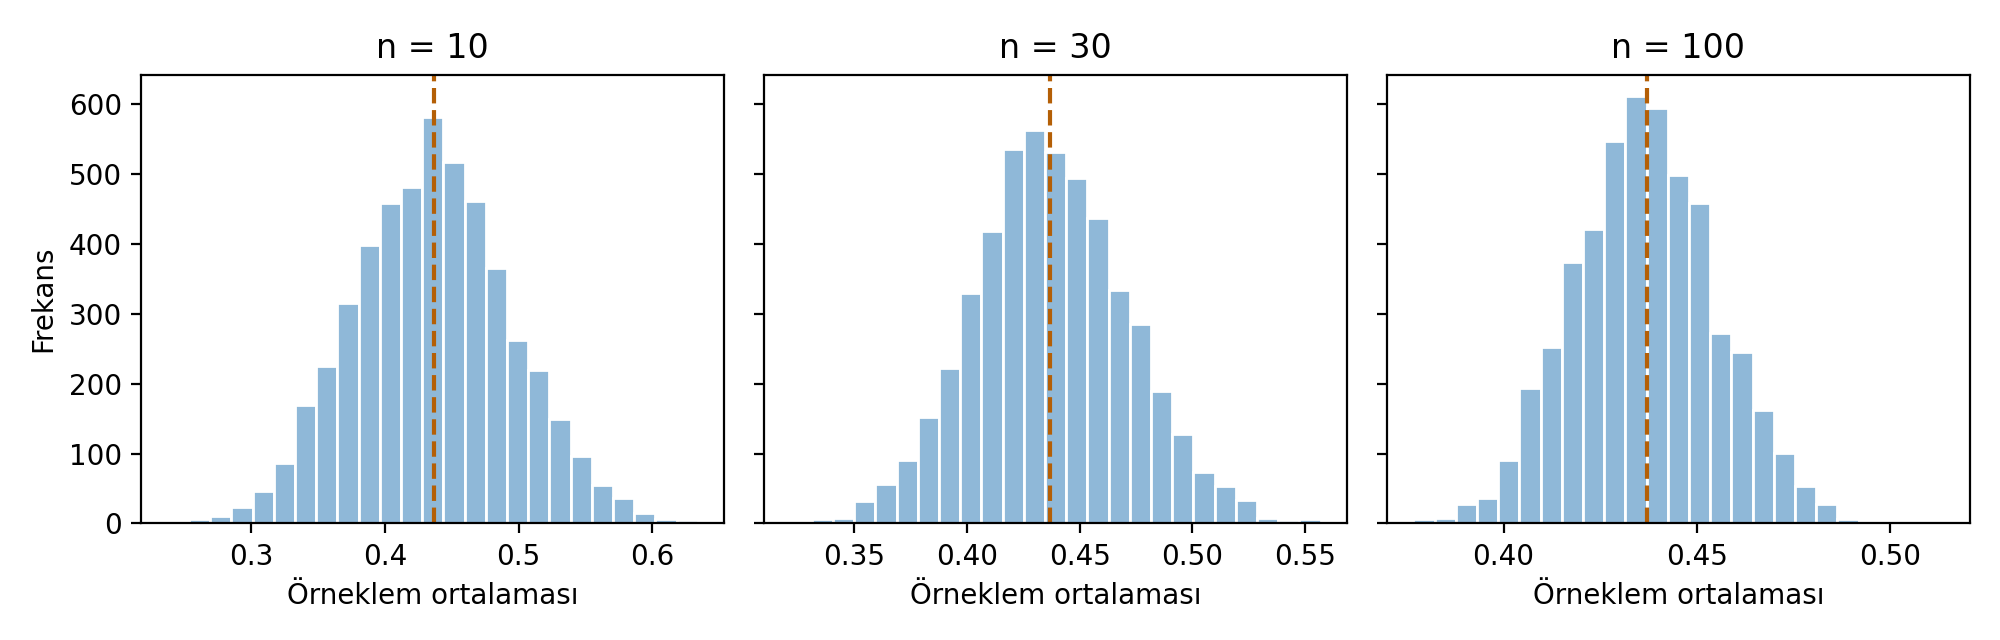
\includegraphics[width=\linewidth]{companion/outputs/figures/chapter04_sampling_means.png}
\caption{B04 için paylaşılan Python histogramları ve normal eğriler.
Sol panel 5, sağ panel 30 çekimin ortalamalarını gösterir;
yatay ve düşey ölçekler ortaktır.}
\label{fig:b04-dogrulanmis-grafikler}
\end{figure}

\Needspace{17\baselineskip}
\begin{outputguidebox}
Tablo~\ref{tab:b04-dogrulanmis-betimsel} ve
Şekil~\ref{fig:b04-dogrulanmis-grafikler}, 30 çekimlik ortalamaların
5 çekimlik ortalamalara göre daha dar dağıldığını gösterir. Buradaki
standart sapma, bireysel öğrenci notlarının değil tekrar ortalamalarının
yayılımıdır. 2.000 tekrar ile örneklem büyüklükleri 5 ve 30 karıştırılmaz.

Paylaşılan SPSS histogramları frekans, R ve Python histogramları
yoğunluk ölçeğindedir. R ve Python'da sınıf genişliği 0,5 ve yatay
aralık 0--20 olsa da sınıf sınırındaki değerlerin yerleştirilme kuralları
farklı olduğundan sütun yükseklikleri birebir eşleşmez. Normal eğriler
görsel karşılaştırma içindir; normalliği kanıtlamaz.

Hazır tekrarlar her ortamda aynıdır; yeniden rastgele çekim
yapılmadığından yazılımlar arasında tohum eşitlemek gerekmez. Hesaplama
uyumu, kaynak öğrenci verisinin daha geniş bir evreni temsil ettiğini
göstermez. Aynı satırdaki iki ortalama ortak çekimler içerir.
\end{outputguidebox}

\textbf{Raporlama örneği (doğrulanmış çıktılarla).}
``Ampirik not dağılımından geri koyarak üretilen 2.000 tekrarda,
5 çekimlik ortalamaların ortalaması 10,367800 ve standart sapması
2,078856; 30 çekimlik ortalamaların ortalaması 10,419050 ve standart
sapması 0,844512 bulunmuştur. Ortak ölçekli histogramlarda 30 çekimlik
ortalamalar daha dar bir dağılım göstermiştir. Sonuçlar yeni öğrenci
gözlemleri değil benzetim çıktılarıdır; iki sütun bağımsız gruplar
olarak test edilmemiştir.''


\textbf{Görev.} İki histogramı aynı yatay ölçekle karşılaştırın. Tek bir
öğrencinin not dağılımı ile örneklem ortalamasının dağılımını ayıran bir
cümle yazın. Geri koyarak çekim nedeniyle burada sonlu evren düzeltmesi
uygulanmadığını açıklayın.

\section{R ile çözümlü uygulama}
\label{sec:r-b04}

\textbf{Soru.} $\{2,4,6,8\}$ evreninden geri koymalı iki çekimin bütün
sıralı sonuçlarını oluşturun. Örneklem ortalamasının dağılımını ve standart
hatasını benzetim hatası olmadan hesaplayın.

\begin{lstlisting}[style=prismR]
evren <- c(2, 4, 6, 8)
ciftler <- expand.grid(ilk = evren, ikinci = evren)
ortalamalar <- rowMeans(ciftler)
frekans <- table(ortalamalar)
data.frame(ortalama = as.numeric(names(frekans)),
           frekans = as.integer(frekans),
           olasilik = as.numeric(frekans) / nrow(ciftler))
merkez <- mean(ortalamalar)
varyans <- mean((ortalamalar - merkez)^2)
c(beklenen_deger = merkez, varyans = varyans,
  standart_hata = sqrt(varyans))
sigma <- sqrt(mean((evren - mean(evren))^2))
sigma / sqrt(2)
barplot(prop.table(frekans), xlab = "Orneklem ortalamasi",
        ylab = "Olasilik")
\end{lstlisting}

\begin{outputguidebox}
\textbf{Çözüm ve kontrol değerleri.} Toplam 16 sıralı örneklem vardır.
2--8 arasındaki ortalamaların frekansları $1,2,3,4,3,2,1$'dir.
Dağılımın beklenen değeri 5, varyansı 2,5 ve standart hatası
$\sqrt{2{,}5}=1{,}5811$'dir. Evren standart sapması $\sqrt{5}$ olduğundan
$\sigma/\sqrt{2}$ aynı sonucu verir.
\end{outputguidebox}

\textbf{Yorum.} Bütün olasılık dağılımı listelendiği için varyans 16 böleni
ile hesaplanır. \texttt{var(ortalamalar)} ise 15'e böler ve burada aranan
tam dağılım varyansını vermez. Geri koymasız seçim bu kodla aynı tasarım değildir.

\textbf{Pekiştirme ve yanıt.} $\P(\bar X\geq7)$ değerini
\texttt{mean(ortalamalar >= 7)} ile bulun: $3/16=0{,}1875$.

\begin{etkinlik}
Bir örnekleme dağılımını yorumlarken üç soruyu yanıtlayın: Dağılımdaki her
nokta neyi temsil ediyor? Merkez hangi parametreyle karşılaştırılıyor?
Genişliği örneklem hacmi ve tasarım nasıl etkiliyor?
\end{etkinlik}

\section{Bölüm özeti}

\begin{itemize}
  \item Örnekleme dağılımının gözlemleri değil, bir istatistiğin tekrarlarını gösterir.
  \item Örneklem ortalaması $\mu$ çevresinde merkezlenir ve varyansı $\sigma^2/n$'dir.
  \item Örneklem oranının standart hatası $\sqrt{p(1-p)/n}$ biçimindedir.
  \item Büyük örneklem değişkenliği azaltır; kötü tasarımdan gelen yanlılığı gidermez.
  \item Örneklem hacminin dört katına çıkması ortalama ve oran standart
  hatalarını yaklaşık yarıya indirir.
  \item Benzetim tekrar sayısı ile her tekrardaki örneklem hacmi farklı
  kavramlardır ve farklı belirsizlik kaynaklarını etkiler.
\end{itemize}

\bolumkaynaklari{\cite{hogg2015,wasserman2004}}

\section*{Alıştırmalar}

\begin{enumerate}
  \item Örnekleme değişkenliğini örnekleme yanlılığından ayırın.
  \item Ham puan dağılımı ile ortalamanın örnekleme dağılımını karşılaştırın.
  \item Örneklem hacmi arttığında $\Var(\bar X)$ nasıl değişir?
  \item $\sigma=18$ ve $n=81$ için $\SE(\bar X)$ değerini bulun.
  \item Büyük örneklemin neden yanlı örnekleme tasarımını düzeltemeyeceğini açıklayın.
  \item $p=0{,}40$ ve $n=100$ için $\SE(\hat p)$ değerini hesaplayın.
  \item Küçük evren örneğinde $\bar X=5$ sonucunu veren dört sıralı örneklemi yazın.
  \item Aynı sınıftan seçilen öğrencilerin bağımsızlık koşulunu neden zayıflatabileceğini açıklayın.
  \item $\mu=80$, $\sigma=16$ ve $n=64$ için $\E[\bar X]$,
  $\Var(\bar X)$ ve $\SE(\bar X)$ değerlerini bulun.
  \item Standart hatayı üçte bire indirmek için örneklem hacminin yaklaşık kaç
  katına çıkarılması gerektiğini gösterin.
  \item $p=0{,}60$ ve $n=600$ için örneklem oranının standart hatasını hesaplayın.
  \item Merkezi gerçek parametreden uzak fakat çok dar bir örnekleme dağılımını
  yanlılık ve değişkenlik bakımından yorumlayın.
  \item Benzetim tekrar sayısını artırmakla örneklem hacmini artırmanın
  sonuçlarını karşılaştırın.
  \item $2,6$ değerlerinden oluşan bir evrenden yerine koyarak iki gözlem
  seçildiğinde örneklem ortalamasının tam dağılımını oluşturun.
\end{enumerate}